\documentclass{llncs}

% A. Objectives
%    1. You should apply one of the techniques studied in the course to
%       solve this problem.
%    2. Devise and perform an empirical evaluation of your system.
%    3. Report your work.
%    4. All your documentation and source code should be available on your GitLab
%       project repository, as well as tasks and milestones. This will be part of
%       the evaluation.
%
% B. Deliverables
%    1. Progress report (by the end of May) describing
%     - selected approach and
%     - general project work plan
%     - group presentation of the report
%    2. Project report
%     - description of the problem
%     - updated material from the progress report
%     - description of your approach
%     - description of the software: installation, requirements and usage notes
%     - empirical evaluation
%    3. Software
%     - application and required libraries/software
%     - brief installation notes (README file)
%    4. Final Presentation
%     - description of your approach
%     - strengths and weaknesses
%     - empirical evaluation
%     - contribution of team members
%
% C. Timeline
%    1. 2018-05-30 Progress report and presentation
%    2. 2018-06-18 Software deliverable and final report
%    3. 2018-06-22 Final Presentation and Demo

\usepackage[utf8]{inputenc}
\usepackage[T1]{fontenc}

\usepackage{geometry}
\geometry{
  a4paper,
  textwidth=16cm,  % llncs has 12.2cm
  textheight=25cm, % llncs has 19.3cm
  heightrounded,
  hratio=1:1,
  vratio=2:3,
}

\usepackage[english]{babel}

\usepackage{hyperref}
\usepackage{bookmark}
\usepackage{csquotes}
\usepackage{multicol}

% In the appendix:
%\usepackage{longtable}
\usepackage{booktabs}

\usepackage{tikz,comment}
\usetikzlibrary{shapes.multipart,positioning,backgrounds}

\pagestyle{plain}

\newcommand{\htw}{\emph{Hunt the Wumpus }}

\title{Hakuna Matata: A Logic-Based Agent for the \htw Game}
\subtitle{Project Report}
\author{Team White\\[2mm]Filippo~De~Bortoli \and Aneta~Koleva \and Lorenz~Leutgeb}
\institute{Free University of Bozen-Bolzano\\[3mm] \texttt{\{\href{mailto:filippo.debortoli@stud-inf.unibz.it}{filippo.debortoli},\href{mailto:aneta.koleva@stud-inf.unibz.it}{aneta.koleva},\href{mailto:lorenz.leutgeb@stud-inf.unibz.it}{lorenz.leutgeb}\}\newline @stud-inf.unibz.it}}

\begin{document}

\maketitle
\thispagestyle{plain}

\begin{abstract}
  The assigned task is to develop an intelligent agent that plays the \htw game, by using a logic-based approach in its implementation.
  In order to complete a run of the game, this agent has to be able to face several challenges, like the incompleteness of the available information about the state of the world or the search for the best strategy to employ.
  The chosen approach is to develop a hybrid agent that relies on an ASP core to actuate its strategy and on graph-theory techniques to obtain additional insights on how to proceed in the exploration of a dungeon.
  To assess the performance of our agent, we implemented an omniscient agent that obtains an optimal score for a given dungeon and we ranked our agent against it.
  In this report, we introduce our solution to this task, by detailing the architecture of the agent and describing the chosen strategy, the heuristics and the obtained results.
\end{abstract}

\section{Problem Statement}
%TODO Define what \htw is, all its rules and constraints.
%TODO Mention that it is also an example in the standard textbook AIMA and thus suited as an exercise in logic-based AI.

\htw is a single player, old computer game which was first released back in 1975. The game is played in the wumpus world(a cave) which is represented as a grid (default size 4x4) and in this world there are few challenges for the player. Each cell on the grid is a room which is connected by passageways with its orthogonally adjacent cell and in one of these cells there is Wumpus, a beast that eats the player if he enters the room. The player has only one arrow, that's one opportunity for shooting the Wumpus. In addition, some of the rooms are bottomless pits and if the player wanders in these rooms it will stay trapped. The main goal of the player is while facing these challenges, to find the hidden gold and leave the cave alive. At the beginning of the game, the player is always positioned on cell [1,1], facing to the right and has 0 points. From here it can use three moves : \textit{Forward, TurnLeft, TurnRight} for discovering its environment and three actions \textit{Shoot, Grab} and \textit{ Climb} for shooting the arrow, grabbing the gold and climbing out of the cave respectively. For each of the moves and actions the player loses 1 point and 10 points when using the arrow. When eaten by the wumpus or trapped in pit, loses 1000 points, and for climbing out of the cave with the gold gains 1000 points. Whenever the player goes to a new cell, it has five sensors that give information about:
\begin{description}
	\item [$\bullet$] Stench - whether the Wumpus is in adjacent cell 
	\item [$\bullet$] Breeze - whether there is a pit in adjacent cell	
	\item [$\bullet$] Glitter - when the gold is in the current cell
	\item [$\bullet$] Bump - whether the player has hit a border
	\item [$\bullet$] Scream- whether the Wumpus is hit by the arrow 
\end{description}
The locations of the gold and the wumpus are chosen randomly with uniform distribution in each cell other then the start. Additionally each cell can be a pit with probability 0.2.

In the book Artificial Intelligence: A Modern Approach, the game is used as an example for representing knowledge-based agents. The environment which represents the Wumpus World is is described as discrete, static, single-agent and partly-observable. For an agent in such environment the main challenge is its initial ignorance of the configuration of the world and using logical reasoning can be helpful for solving this. 



\section{Approach}
% This should be a high-level section that does not really talk too much
% about code (for that we have the "Implementation" section), but instead
% about the general approach.
\subsection{ASP technique}
For the purpose of this project, we decided to implement an intelligent agent that plays the wumpus game using ASP technique in combination with graph-theory techniques to explore the search space and find its best strategy for finishing the game with maximum points. The environment in which the agent is playing is discrete and static, since the wumpus, the gold and the pits are all fixed. The agent's initial knowledge base contains the rules of the game without specifying the size of the grid. The size is discovered by the agent when it hits a border and the 'Bump' percept is on, after which the agent knows how big the search space it is. In order to be able to find the best strategy, the agent first needs to acquire certain knowledge about the search space and to be able to reason wrt this knowledge. The facts and rules in the knowledge base are specified as ASP rules and DVL solver is used for grounding and solving. One of the advantages of ASP is the fact that it uses non-monotonic reasoning and closed world assumption which allow the agent to correctly derive what is logically right from it's knowledge base. Moreover DLV is able to process incomplete knowledge which the agent has while overcoming its initial ignorance with logical reasoning. 

%TODO Justify why we chose ASP (non-monotonic reasoning, fits nicely with incomplete knowledge), previous experience with it, easier to write high-level logic thanks to grounding. 
% maybe mention that we can write strong constraints, not sure if still have that

\subsection{A* search algorithm}
For better exploration of the world, we build a graph that represents reachability (with cost) for all cells. Then we use \textit{Manhattan distance} as a cost function for calculating the cost from the current cell to the next cell. 
For calculating the minimal cost of reaching the goal cell we use \textit{A* search algorithm} : \(f(n) = g(n) + h(n)\).
In our program \(g(n)\) represents the cost of the path from the current cell to the next cell \(n\), and \(h(n)\) represents the heuristic estimated cost of the cheapest path from cell \(n\) to the goal cell.  

%TODO How does our agent explore the world (A*-search)
%not sure if here should be explained the purpose of pathTurnCost,
%departureTurnCost and rotCost or leave that for implementation

\subsection{Different modes}
While playing, our agent can be in 1 from 4 available modes at any time. When the game starts, the first mode of the agent is \textit{explore}. It stays in this mode until it discovers the gold or there are cell which haven't been explored yet. Once the agent is in the cell where the gold is, its next action is to grab the gold and in this moment is in mode \textit{grab}. If there are no more cells safe for exploration, the gold is not grabbed and the agent is facing the wumpus, the mode switches to \textit{kill}. The last available mode is \textit{escape}, in which the agent is if it's not in any of the other three modes. The agent is in this mode after grabbing the gold or after not being able to explore any other cells and leaves the cave empty handed.

%TODO Describe the modes that we extracted from the gameplay and what are the conditions that make the agent switch modes.

%TODO Describe the high level approach

\begin{center}
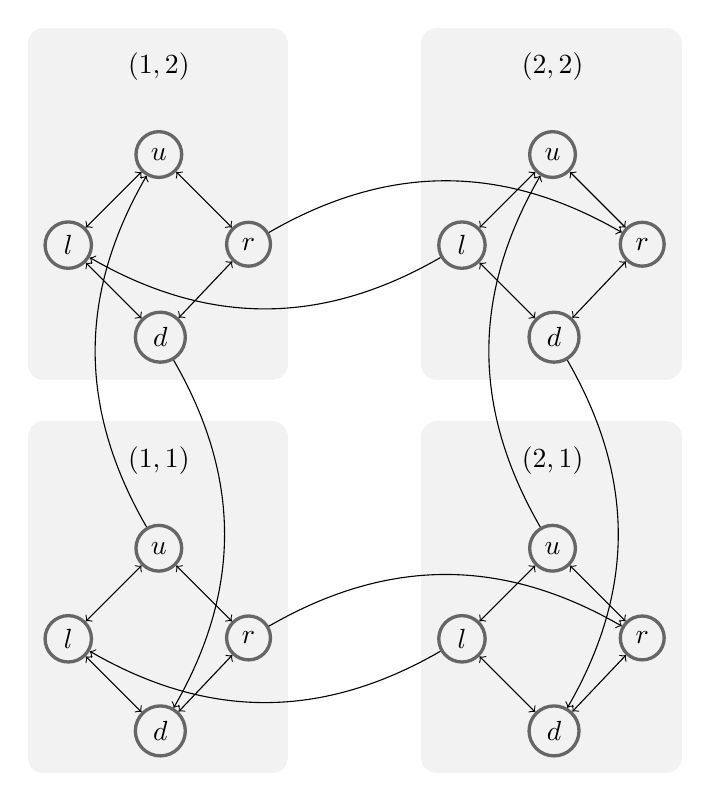
\begin{tikzpicture}[roundnode/.style={circle, draw=black!60, very thick,minimum size=4mm}]
	\begin{scope}
	    \node (n11) {$(1, 1)$};
		\node[roundnode] (u11) [below=5mm of n11] {$u$};
		\node[roundnode] (l11) [below left=10mm of u11] {$l$};
		\node[roundnode] (r11) [below right=10mm of u11] {$r$};
		\node[roundnode] (d11) [below right=10mm of l11] {$d$};
		\draw [<->] (u11) -> (l11);
		\draw [<->] (u11) -> (r11);
		\draw [<->] (d11) -> (l11);
		\draw [<->] (d11) -> (r11);
	\end{scope}

	\begin{scope}[xshift=5cm]
	    \node (n21) {$(2, 1)$};
		\node[roundnode] (u21) [below=5mm of n21] {$u$};
		\node[roundnode] (l21) [below left=10mm of u21] {$l$};
		\node[roundnode] (r21) [below right=10mm of u21] {$r$};
		\node[roundnode] (d21) [below right=10mm of l21] {$d$};
		\draw [<->] (u21) -> (l21);
		\draw [<->] (u21) -> (r21);
		\draw [<->] (d21) -> (l21);
		\draw [<->] (d21) -> (r21);
	\end{scope}

	\begin{scope}[yshift=5cm]
	    \node (n12) {$(1, 2)$};
		\node[roundnode] (u12) [below=5mm of n12] {$u$};
		\node[roundnode] (l12) [below left=10mm of u12] {$l$};
		\node[roundnode] (r12) [below right=10mm of u12] {$r$};
		\node[roundnode] (d12) [below right=10mm of l12] {$d$};
		\draw [<->] (u12) -> (l12);
		\draw [<->] (u12) -> (r12);
		\draw [<->] (d12) -> (l12);
		\draw [<->] (d12) -> (r12);
	\end{scope}

	\begin{scope}[yshift=5cm,xshift=5cm]
	    \node (n22) {$(2, 2)$};
		\node[roundnode] (u22) [below=5mm of n22] {$u$};
		\node[roundnode] (l22) [below left=10mm of u22] {$l$};
		\node[roundnode] (r22) [below right=10mm of u22] {$r$};
		\node[roundnode] (d22) [below right=10mm of l22] {$d$};
		\draw [<->] (u22) -> (l22);
		\draw [<->] (u22) -> (r22);
		\draw [<->] (d22) -> (l22);
		\draw [<->] (d22) -> (r22);
	\end{scope}

	\path [->] (r11) edge [bend left] (r21);
	\path [->] (l21) edge [bend left] (l11);
	\path [->] (u11) edge [bend left] (u12);
	\path [->] (d12) edge [bend left] (d11);
	\path [->] (u21) edge [bend left] (u22);
	\path [->] (d22) edge [bend left] (d21);
	\path [->] (r12) edge [bend left] (r22);
	\path [->] (l22) edge [bend left] (l12);

	\begin{pgfonlayer}{background}
		\filldraw[line width=4mm,join=round,black!5]
			(n11.north -| r11.east) rectangle (d11.south -| l11.west)
			(n21.north -| r21.east) rectangle (d21.south -| l21.west)
			(n12.north -| r12.east) rectangle (d12.south -| l12.west)
			(n22.north -| r22.east) rectangle (d22.south -| l22.west);
	\end{pgfonlayer}
\end{tikzpicture}
\end{center}

\section{Implementation}
%TODO Short section where we describe the system, referring to the appendix (see below)
%TODO as well as that we used DLV.
%TODO Generate and include the Dependency Graph
%TODO Autopilot (if it works at some point)
%TODO Refer to usage file for actually running the system.

In this section, we briefly describe how the agent described in the previous section was implemented. Note, however that for the implementation in its full detail we refer to Appendix \ref{hunt-the-wumpus}.

\begin{figure}
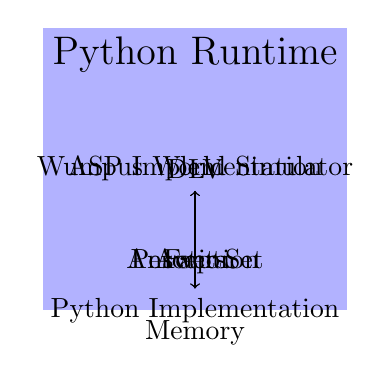
\begin{tikzpicture}
% py and sim should be inside pyr
% mem should be inside py
% asp should be inside dlv

\node[fill=blue!30,text depth = 3cm,minimum width=3cm,font=\Large] (pyr) {Python Runtime};
\node (sim) at (pyr.center) {Wumpus World Simulator};
\node (py) at (pyr.south) {Python Implementation};
\node (mem) at (py.south) {Memory};

\node (dlv) {DLV};
\node (asp) {ASP Implementation};

\draw [->] (py) -> (asp) node [midway, below] {Facts};
\draw [->] (asp) -> (py) node [midway, below] {Answer Set};

\draw [->] (py) -> (sim) node [midway, below] {Action};
\draw [->] (sim) -> (py) node [midway, below] {Perception};
\end{tikzpicture}
\end{figure}

\section{Evaluation}

%TODO mention that we used randomly generated instances:

\begin{tabular}{ccc}
$n$ & $N_n$ \\
4 & 120 \\
5 &  20 \\
6 &  20 \\
7 &  20 \\
8 &  20 \\
\end{tabular}

%TODO maybe more instances?

%TODO We implemented an agent that solves the instances with perfect information to compare against.

%\section{Introduction}

% TODO
%
% - describe the task that has been solved
% - outline structure of the report 
%\section{Installation and Usage}
\label{sec:usage}

\subsection{An example}
%\input{sections/strategy}
%\section{Evaluation}

% TODO
%
% - describe the structure of the test suite
% - is it necessary to describe machine specs for tests run?
%    I don't think so, we are not checking CPU time or machine-related data. ~Filippo
% - describe collected data (variables, clauses, models, ...)
% - desiderata: plot describing evolution of different versions of the front-end
% - arrogant: comparisons with data from other teams on same test suite.

\newpage

\appendix
\footnotesize

\begin{multicols}{2}
\hypertarget{hunt-the-wumpus}{%
\section{Hunt the Wumpus}\label{hunt-the-wumpus}}

This is an implementation of an agent that plays ``Hunt the Wumpus''.

Input should be given as follows:

\begin{verbatim}
#maxint = 1000.
\end{verbatim}

\hypertarget{constants}{%
\subsection{Constants}\label{constants}}

We use constants to encode concrete orientations, actions and modes, and
one corresponding predicate to all of them respectively.

According to \texttt{wumpus.common.Orientation} we define orientations.

\begin{verbatim}
#const right = 0.
#const up    = 1.
#const left  = 2.
#const down  = 3.

isOrientation 0..3
\end{verbatim}

According to \texttt{wumpus.common.Action} we define actions.

\begin{verbatim}
#const goforward = 0.
#const turnleft  = 1.
#const turnright = 2.
#const grab      = 3.
#const shoot     = 4.
#const climb     = 5.

isAction 0..5
\end{verbatim}

According to \texttt{wumpus.agent.Mode} we define modes.

\begin{verbatim}
#const explore = 0.
#const escape  = 1.
#const kill    = 2.

isMode 0..3
\end{verbatim}

Additionally we designate two orthogonal orientations as axes.

\begin{verbatim}
axis right
axis up
\end{verbatim}

Being able to mirror orientations/turns will come in handy.

\begin{verbatim}
mirror         left right
mirror         up   down
mirror         O2   O1
        mirror O1   O2
\end{verbatim}

\hypertarget{world-size}{%
\subsection{World Size}\label{world-size}}

If the agent never bumped against a wall, it has no information about
the size of the world.

\begin{verbatim}
sizeKnown
        bump _ _
\end{verbatim}

We will therefore derive the size of the world from something already
known.

\begin{verbatim}
exploredSize     X
        explored X Y

exploredSize       Y
        explored X Y
\end{verbatim}

Since any cell we already explored certainly is part of the world, we
can use this information and guess that the world is ``just a little''
bigger than we already know.

\begin{verbatim}
size                            S
        not sizeKnown
        #succ             Sm    S
        #max              Sm Se
                exploredSize Se
\end{verbatim}

Of course, if the agent bumped, the size can be directly inferred.

\begin{verbatim}
size               S
        bump  Sm Y
        >     Sm Y
        #prec Sm   S

size               S
        bump  X Sm
        <=    X Sm
        #prec   Sm S
\end{verbatim}

\hypertarget{cells-neighbors-facing-and-bumps}{%
\subsection{Cells, Neighbors, Facing And
Bumps}\label{cells-neighbors-facing-and-bumps}}

Span the space of cells.

\begin{verbatim}
cell         X Y
        #int X
        #int   Y
        >      Y 0
        >    X   0
        <=     Y S
        <=   X   S
        size     S

corner 1 1

corner       X 1
        cell X 1
        size X
        sizeKnown

corner       1 Y
        cell 1 Y
        size   Y
        sizeKnown

corner       S S
        cell S S
        size S
        sizeKnown
\end{verbatim}

Two cells are different if any of the components X, Y are unequal.

\begin{verbatim}
diff         X1 Y1 X2 Y2
        cell X1 Y1
        cell       X2 Y2
        !=   X1    X2

diff         X1 Y1 X2 Y2
        cell X1 Y1
        cell       X2 Y2
        !=      Y1    Y2
\end{verbatim}

\hypertarget{distances-and-costs}{%
\subsubsection{Distances and Costs}\label{distances-and-costs}}

The two predicates \texttt{outgoing} and \texttt{incoming} will help us
to keep the space for which we have to compute costs small.

\begin{verbatim}
neighborhood              X2 Y2
        now         X1 Y1       _
        anyNeighbor X1 Y1 X2 Y2
        safe              X2 Y2

outgoing             X Y
        neighborhood X Y

outgoing     X Y
        now  X Y _

incoming     X Y
        safe X Y
\end{verbatim}

We define distance along axes

\begin{verbatim}
distAlong        X1 Y1 X2 Y2 right D
        cell     X1 Y1
        cell           X2 Y2
        #absdiff       X1 X2       D

distAlong        X1 Y1 X2 Y2 up D
        #absdiff       Y1 Y2    D
        cell     X1 Y1
        cell           X2 Y2
\end{verbatim}

And using that, manhattan/taxicab distance is a charm.

\begin{verbatim}
manhattan            X1 Y1 X2 Y2             M
        outgoing     X1 Y1
        distAlong    X1 Y1 X2 Y2 right D1
        distAlong    X1 Y1 X2 Y2 up    D2
        +                              D1 D2 M

pathTurnCost          X Y O X Y 0
        outgoing  X Y
        isOrientation     O

pathTurnCost          X1 Y1 O1 X2 Y2 0
        isOrientation       O1
        facing        X1 Y1 _ X2 Y2
        diff          X1 Y1   X2 Y2

pathTurnCost             X1 Y1 O1 X2 Y2 1
        outgoing         X1 Y1
        isOrientation          O1
        incoming                  X2 Y2
        not pathTurnCost X1 Y1 O1 X2 Y2 0

departureTurnCost        X1 Y1 O1 X2 Y2    C
        outgoing     X1 Y1
        isOrientation          O1
        incoming                  X2 Y2
        #min                               C Cm
                reach    X1 Y1    X2 Y2 O2
                turnCost       O1       O2   Cm

rotCost                   X1 Y1 O1 X2 Y2       C
        outgoing          X1 Y1
        isOrientation           O1
        incoming                   X2 Y2
        pathTurnCost      X1 Y1 O1 X2 Y2 Cp
        departureTurnCost X1 Y1 O1 X2 Y2    Cd
        +                                Cp Cd C
\end{verbatim}

We use the Manhattan distance as cost function.

\begin{verbatim}
cost                      X1 Y1 O1 X2 Y2 C
        outgoing          X1 Y1
        isOrientation           O1
        incoming                   X2 Y2
        rotCost           X1 Y1 O1 X2 Y2 Cr
        manhattan         X1 Y1    X2 Y2    Cm
        +                                Cr Cm C
\end{verbatim}

The turn predicate associates two orientations with the action that must
be taken in order to turn from the first orientation to the second (if
possible).

\begin{verbatim}
turn up    left  turnleft
turn left  down  turnleft
turn down  right turnleft
turn right up    turnleft

turn up    right turnright
turn down  left  turnright
turn left  up    turnright
turn right down  turnright

turnCost              O O 0
        isOrientation O

turnCost                  O1 O2 1
            isOrientation O1
            isOrientation     O2
            !=            O1 O2
        not mirror        O1 O2

turnCost               O1 O2 2
        isOrientation  O1
        isOrientation     O2
        mirror         O1 O2
\end{verbatim}

Neighboring cells along the horizontal and vertical axis.

\begin{verbatim}
neighbor      X1 Y X2 Y right
        cell  X1 Y
        cell       X2 Y
        #succ X1   X2

neighbor      X Y1 X Y2 up
        cell  X Y1
        cell       X Y2
        #succ   Y1   Y2

neighbor         X1 Y1 X2 Y2 O2
        neighbor X2 Y2 X1 Y1 O1
        mirror               O1 O2

anyNeighbor           X1 Y1 X2 Y2
        neighbor      X1 Y1 X2 Y2 O
        isOrientation             O

twoNeighbors        X1 Y1 X2 Y2 X3 Y3
        anyNeighbor X1 Y1 X2 Y2
        anyNeighbor X1 Y1       X3 Y3
        diff              X2 Y2 X3 Y3

square               X1 Y1 X2 Y2 X3 Y3 X4 Y4
        twoNeighbors X1 Y1 X2 Y2 X3 Y3
        twoNeighbors X4 Y4 X2 Y2 X3 Y3
        diff         X1 Y1             X4 Y4

triple           X1 Y1 X2 Y2 X3 Y3
        neighbor X1 Y1 X2 Y2       A
        neighbor       X2 Y2 X3 Y3 A
        diff     X1 Y1       X3 Y3
        axis                       A
\end{verbatim}

Cells that agree on one component.

\begin{verbatim}
facing       X Z up X Y
        cell X Z
        <      Z      Y
        cell X        Y

facing       Z Y right X Y
        cell           X Y
        <    Z         X
        cell Z           Y

facing         X2 Y2    O2 X1 Y1
        facing X1 Y1 O1    X2 Y2
        mirror       O1 O2

reach        X1 Y1 X2 Y2 right
        cell X1 Y1
        cell       X2 Y2
        <    X1    X2

reach        X1 Y1 X2 Y2 up
        cell X1 Y1
        cell       X2 Y2
        <       Y1    Y2

reach        X1 Y1 X2 Y2 left
        cell X1 Y1
        cell       X2 Y2
        >    X1    X2

reach        X1 Y1 X2 Y2 down
        cell X1 Y1
        cell       X2 Y2
        >       Y1    Y2
\end{verbatim}

Complete information about information. We only do this here and not in
Python since we might have assumed a size.

\begin{verbatim}
-explored            X Y
        cell         X Y
        not explored X Y
\end{verbatim}

\hypertarget{do}{%
\subsection{Do}\label{do}}

\begin{verbatim}
priority
        shouldShoot

priority
        shouldClimb

priority
        shouldGrab

priority
        shouldAim

do shoot
        shouldShoot

do grab
        shouldGrab

do climb
        shouldClimb

do              A
        succAim A

do                   A
            towards  A
        not priority

shouldShoot
        mode   kill
        now    X Y O
        attack X Y O
\end{verbatim}

Pick gold if there's some in the cell, independently of the current
mode.

\begin{verbatim}
shouldGrab
        now     X Y O
        glitter X Y
\end{verbatim}

Climb if gold is picked and back to initial cell.

\begin{verbatim}
shouldClimb
        now 1 1 O
        mode escape
\end{verbatim}

Generally we will be turning and go forward towards a goal. Exceptions
are when we want to take high priority actions like grabbing, climbing
or shooting.

\begin{verbatim}
canFace                          A
        facing X1 Y1    O2 X2 Y2
        now    X1 Y1 O1
        next               X2 Y2
        !=           O1 O2
        turn         O1 O2       A

-cannotFace
        isAction A
        canFace  A

cannotFace
        not -cannotFace

towards goforward
        facing X1 Y1 O1 X2 Y2
        now    X1 Y1 O1
        next            X2 Y2

towards         A
        canFace A
        not towards goforward
\end{verbatim}

TODO: Can we turn in a better way?

\begin{verbatim}
towards turnleft
        not towards goforward
        cannotFace
\end{verbatim}

\hypertarget{detection-of-wumpus}{%
\subsection{Detection Of Wumpus}\label{detection-of-wumpus}}

\begin{verbatim}
wumpus         X1 Y1
        square X1 Y1 X2 Y2 X3 Y3 X4 Y4
        stench       X2 Y2
        stench             X3 Y3
        explored                 X4 Y4
        -wumpusDead
\end{verbatim}

Antipodal matching.

\begin{verbatim}
wumpus               X2 Y2
        triple X1 Y1 X2 Y2 X3 Y3
        stench X1 Y1
        stench             X3 Y3
        -wumpusDead
\end{verbatim}

Corner case.

\begin{verbatim}
wumpus                     XW YW
        twoNeighbors XC YC XW YW XE YE
        stench       XC YC
        corner       XC YC
        explored                 XE YE
        -wumpusDead
\end{verbatim}

Auxiliary flag to signal detection of wumpus.

\begin{verbatim}
wumpusDetected
        cell  X Y
        wumpus X Y
\end{verbatim}

If wumpus is not certainly detected, we must exclude other cells where
it might be.

\begin{verbatim}
possibleWumpus            X2 Y2
        anyNeighbor X1 Y1 X2 Y2
        stench      X1 Y1
        -explored         X2 Y2
        not shotAt        X2 Y2
        -wumpusDead
        not wumpusDetected

shotAt                  X Y
        facing XS YS OS X Y
        shot   XS YS OS
\end{verbatim}

\hypertarget{detection-of-pits}{%
\subsection{Detection Of Pits}\label{detection-of-pits}}

A neighbor of a breeze is a possible pit if it can be.

\begin{verbatim}
possiblePit         XB YB XP YP
        breeze      XB YB
        anyNeighbor XB YB XP YP
        not -pit          XP YP
\end{verbatim}

Any explored cell certainly cannot be a pit, otherwise we would be dead
by now.

\begin{verbatim}
-pit             X Y
        explored X Y
\end{verbatim}

If we have explored a cell already and felt no brezee, then no neighbor
can be a pit.

\begin{verbatim}
-pit                      X2 Y2
        anyNeighbor X1 Y1 X2 Y2
        -breeze     X1 Y1
\end{verbatim}

Finally, we assume that there are pits where there might be possible
pits.

\begin{verbatim}
pit                     X Y
        possiblePit _ _ X Y
\end{verbatim}

\hypertarget{safety-of-cells}{%
\subsection{Safety Of Cells}\label{safety-of-cells}}

Any cell where the wumpus is is not safe.

\begin{verbatim}
safe             X Y
        explored X Y

-safe          X Y
        wumpus X Y

-safe                  X Y
        possibleWumpus X Y

-safe       X Y
        pit X Y

safe              X Y
        reachable X Y
        not -safe X Y
\end{verbatim}

\hypertarget{explore-mode}{%
\subsection{Explore Mode}\label{explore-mode}}

\begin{verbatim}
reachable           X Y
        anyNeighbor X Y XE YE
        explored        XE YE

reachable        X Y
        explored X Y
\end{verbatim}

Auxiliary flag to signal whether we can still explore further.

\begin{verbatim}
frontier          X Y
        reachable X Y
        safe      X Y
        -explored X Y

shouldExplore
        frontier X Y
\end{verbatim}

\hypertarget{kill-mode}{%
\subsection{Kill Mode}\label{kill-mode}}

\begin{verbatim}
dontShoot
        possibleWumpus X Y
        pit            X Y

dontShoot
        wumpus X Y
        pit    X Y

dontShoot
        not haveArrow

dontShoot
        wumpusDead

dontShoot
        grabbed

canKill        XS YS OS
        facing XS YS OS XW YW
        wumpus          XW YW
        safe   XS YS

shouldKill
        canKill _ _ _
        not dontShoot

canTryKill       X Y O
        facing   X Y O XC YC
        safe     X Y
        possibleWumpus XC YC

shouldTryKill
            canTryKill _ _ _
        not shouldKill
        not dontShoot

attack             X Y O
        canTryKill X Y O
        shouldTryKill

attack          X Y O
        canKill X Y O
        shouldKill

shouldAttack
        attack _ _ _

aim                        OS
            !=           O OS
            attack XS YS   OS
        not attack XS YS O
            now    XS YS O

canAim                A
        turn    O1 O2 A
        aim        O2
        now _ _ O1

-cannotAim
        canAim _

cannotAim
        not -cannotAim

succAim        A
        canAim A
        mode   kill

succAim turnleft
        aim _
        cannotAim
        mode kill

shouldAim
        succAim A
\end{verbatim}

\hypertarget{optimization-for-goal}{%
\subsection{Optimization For Goal}\label{optimization-for-goal}}

\begin{verbatim}
h                     X2 Y2 C
        cost X1 Y1 O1 X2 Y2 C
        now  X1 Y1 O1
\end{verbatim}

Interesting candidates are those cells that we have not yet explored and
we know that they are safe.

\begin{verbatim}
candidate 1      X Y C
        h        X Y C
        frontier X Y
        mode     explore

candidate 1    X Y C
        h      X Y C
        attack X Y _
        mode   kill

candidate 1 1 1 C
        h   1 1 C
        mode escape

candidate 2                     X Y         C
        now         XN YN ON
        anyNeighbor XN YN   X Y
        safe                X Y
        goal                      XG YG
        cost                X Y O XG YG C2
        reach       XN YN X Y O
        + C1 C2 C
        + Cr 1 C1
        departureTurnCost XN YN ON X Y Cr
        not easyGoal

candidate      2 X Y C
        choice 1 X Y C
        easyGoal

level 1
level 2

next X Y
        choice 2 X Y C

goal X Y
        choice 1 X Y C

easyGoal
        now         XN YN _
        anyNeighbor XN YN XG YG
        goal              XG YG

foundNext
        next _ _
\end{verbatim}

TODO: Inconsistent? - foundGoal not foundNext

\begin{verbatim}
foundGoal
        goal _ _
\end{verbatim}

TODO: Inconsistent? - not foundGoal not priority

\begin{verbatim}
choice L X Y C | -choice L X Y C
        level     L
        candidate L X Y C

~
        level     L
        candidate L X1 Y1 C1
        candidate L          X2 Y2 C2
        choice    L          X2 Y2 C2
        <=                C1       C2
\end{verbatim}

\hypertarget{autopilot}{%
\subsection{Autopilot}\label{autopilot}}

\begin{verbatim}
-autopilot
        not autopilot

autopilot
        not priority
        mode explore

autopilot
        not priority
        mode escape
\end{verbatim}

\hypertarget{mode-selector}{%
\subsection{Mode Selector}\label{mode-selector}}

\begin{verbatim}
mode grab
        shouldGrab

mode explore
         not mode grab
        shouldExplore
        -grabbed

mode kill
        not mode grab
        not mode explore
        shouldAttack
        -grabbed

mode escape
        not mode grab
        not mode explore
        not mode kill
\end{verbatim}

\hypertarget{consistency}{%
\subsection{Consistency}\label{consistency}}

\begin{verbatim}
wouldBump
        now _ 1 down

wouldBump
        now 1 _ left

wouldBump
        size S
        now  _ S up

wouldBump
        size S
        now  S _ right

inSomeMode
        isMode M
        mode   M

doingSomething
        isAction A
        do       A

breezeHasPossiblePit XB YB
        breeze       XB YB
        possiblePit  XB YB _ _
\end{verbatim}

0 We should not go forward, since that would be our second time to bump.

\begin{verbatim}
bad 0
        do goforward
        wouldBump
\end{verbatim}

2 Don't shoot if the wumpus is already dead!

\begin{verbatim}
bad 2
        do shoot
        wumpusDead
\end{verbatim}

3 The agent is not ubiquitous.

\begin{verbatim}
bad 3
        now X Y _
        now X Z _
        !=  Y Z

bad 3
        now X Y _
        now Z Y _
        !=  X Z
\end{verbatim}

4 We cannot be in more than one mode.

\begin{verbatim}
bad 4
        mode X
        mode   Y
        !=   X Y
\end{verbatim}

5 We must be in one mode.

\begin{verbatim}
bad 5
        not inSomeMode
\end{verbatim}

6 We cannot do two things.

\begin{verbatim}
bad 6
        do A1
        do    A2
        != A1 A2
\end{verbatim}

7 We must do something.

\begin{verbatim}
bad 7
        not doingSomething
\end{verbatim}

8 Wumpus detection must be accurate. There is only one wumpus.

\begin{verbatim}
bad 8
        wumpus X1 Y1
        wumpus       X2 Y1
        !=     X1    X2

bad 8
        wumpus X1 Y1
        wumpus X1    Y2
        !=        Y1 Y2
\end{verbatim}

10 There is a cell outside of the world. Whut?

\begin{verbatim}
bad 10
        cell X Y
        >    X   S
        size     S

bad 10
        cell X Y
        >      Y S
        size     S
\end{verbatim}

11 A breeze must have at least one possiblePit.

\begin{verbatim}
bad 11
        breeze                   XB YB
        not breezeHasPossiblePit XB YB
\end{verbatim}

12 explored/2 and notExplored/2 must be disjoint!

\begin{verbatim}
bad 12
        explored    X Y
        notExplored X Y
\end{verbatim}

13 A cell cannot be -safe and explored.

\begin{verbatim}
bad 13
        cell     X Y
        -safe    X Y
        explored X Y
\end{verbatim}

14 We are in explore mode, have no triggers to climb or shoot, but still
did not find a goal.

\begin{verbatim}
bad 14
        not foundGoal
        not shouldGrab
        not shouldClimb
        mode explore
\end{verbatim}

15 We are shooting even though we do not have the arrow anymore.

\begin{verbatim}
bad 15
        do shoot
        -haveArrow
\end{verbatim}

16 Cost function must be decisive.

\begin{verbatim}
bad 16
        cost X Y O X2 Y2 C1
        cost X Y O X2 Y2    C2
        !=               C1 C2
\end{verbatim}

17 Rotation cost must be decisive.

\begin{verbatim}
bad 17
        rotCost X1 Y1 O1 X2 Y2 C1
        rotCost X1 Y1 O1 X2 Y2    C2
        !=                     C1 C2
\end{verbatim}

\end{multicols}

\end{document}
